
\documentclass[
	% -- opções da classe memoir --
	article,			% indica que é um artigo acadêmico
	11pt,				% tamanho da fonte
	oneside,			% para impressão apenas no recto. Oposto a twoside
	a4paper,			% tamanho do papel. 
	% -- opções da classe abntex2 --
	%chapter=TITLE,		% títulos de capítulos convertidos em letras maiúsculas
	%section=TITLE,		% títulos de seções convertidos em letras maiúsculas
	%subsection=TITLE,	% títulos de subseções convertidos em letras maiúsculas
	%subsubsection=TITLE % títulos de subsubseções convertidos em letras maiúsculas
	% -- opções do pacote babel --
	english,			% idioma adicional para hifenização
	brazil,				% o último idioma é o principal do documento
	sumario=tradicional
	]{abntex2}

\usepackage{lmodern}			% Usa a fonte Latin Modern
\usepackage[T1]{fontenc}		% Selecao de codigos de fonte.
\usepackage[utf8]{inputenc}		% Codificacao do documento (conversão automática dos acentos)
\usepackage{indentfirst}		% Indenta o primeiro parágrafo de cada seção.
\usepackage{nomencl} 			% Lista de simbolos
\usepackage{color}				% Controle das cores
\usepackage{graphicx}			% Inclusão de gráficos
\graphicspath{{imagens/}}
\usepackage{microtype} 			% para melhorias de justificação
\usepackage{float}
\usepackage{listingsutf8}
\usepackage{color}

\definecolor{mygreen}{rgb}{0,0.6,0}
\definecolor{mygray}{rgb}{0.5,0.5,0.5}
\definecolor{mymauve}{rgb}{0.58,0,0.82}

\lstset{ %
  backgroundcolor=\color{white},   % choose the background color; you must add \usepackage{color} or \usepackage{xcolor}
  basicstyle=\footnotesize,        % the size of the fonts that are used for the code
  breakatwhitespace=false,         % sets if automatic breaks should only happen at whitespace
  breaklines=true,                 % sets automatic line breaking
  captionpos=b,                    % sets the caption-position to bottom
  commentstyle=\color{mygreen},    % comment style
  deletekeywords={...},            % if you want to delete keywords from the given language
  escapeinside={\%*}{*)},          % if you want to add LaTeX within your code
  extendedchars=true,              % lets you use non-ASCII characters; for 8-bits encodings only, does not work with UTF-8
  frame=single,	                   % adds a frame around the code
  keepspaces=true,                 % keeps spaces in text, useful for keeping indentation of code (possibly needs columns=flexible)
  keywordstyle=\color{blue},       % keyword style
  language=Octave,                 % the language of the code
  otherkeywords={*,...},           % if you want to add more keywords to the set
  numbers=left,                    % where to put the line-numbers; possible values are (none, left, right)
  numbersep=5pt,                   % how far the line-numbers are from the code
  numberstyle=\tiny\color{mygray}, % the style that is used for the line-numbers
  rulecolor=\color{black},         % if not set, the frame-color may be changed on line-breaks within not-black text (e.g. comments (green here))
  showspaces=false,                % show spaces everywhere adding particular underscores; it overrides 'showstringspaces'
  showstringspaces=false,          % underline spaces within strings only
  showtabs=false,                  % show tabs within strings adding particular underscores
  stepnumber=2,                    % the step between two line-numbers. If it's 1, each line will be numbered
  stringstyle=\color{mymauve},     % string literal style
  tabsize=2,	                   % sets default tabsize to 2 spaces
  title=\lstname                   % show the filename of files included with \lstinputlisting; also try caption instead of title
}

		
% ---
% Pacotes de citações
% ---
\usepackage[brazilian,hyperpageref]{backref}	 % Paginas com as citações na bibl
\usepackage[alf]{abntex2cite}	% Citações padrão ABNT
% ---

% ---
% Configurações do pacote backref
% Usado sem a opção hyperpageref de backref
\renewcommand{\backrefpagesname}{Citado na(s) página(s):~}
% Texto padrão antes do número das páginas
\renewcommand{\backref}{}
% Define os textos da citação
\renewcommand*{\backrefalt}[4]{
	\ifcase #1 %
		Nenhuma citação no texto.%
	\or
		Citado na página #2.%
	\else
		Citado #1 vezes nas páginas #2.%
	\fi}%
% ---

% ---
% Informações de dados para CAPA e FOLHA DE ROSTO
% ---
\titulo{Trabalho Prático 5 \\ Algoritmo EM}
\autor{Alisson Moreira Ferreira - 11/0106946 \and Augusto Cesar Ribeiro Nunes - 13/0103004}
\local{Brasília, Brasil}
\data{junho de 2016}
% ---

% ---
% Configurações de aparência do PDF final

% alterando o aspecto da cor azul
\definecolor{blue}{RGB}{41,5,195}

% informações do PDF
\makeatletter
\hypersetup{
     	%pagebackref=true,
		pdftitle={\@title}, 
		pdfauthor={\@author},
    	pdfsubject={Modelo de artigo cientifico com abnTeX2},
	    pdfcreator={LaTeX with abnTeX2},
		pdfkeywords={abnt}{latex}{abntex}{abntex2}{atigo cientifico}, 
		colorlinks=true,       		% false: boxed links; true: colored links
    	linkcolor=blue,          	% color of internal links
    	citecolor=blue,        		% color of links to bibliography
    	filecolor=magenta,      		% color of file links
		urlcolor=blue,
		bookmarksdepth=4
}
\makeatother
% --- 

% ---
% compila o indice
% ---
\makeindex
% ---

% ---
% Altera as margens padrões
% ---
\setlrmarginsandblock{3cm}{3cm}{*}
\setulmarginsandblock{3cm}{3cm}{*}
\checkandfixthelayout
% ---

% --- 
% Espaçamentos entre linhas e parágrafos 
% --- 

% O tamanho do parágrafo é dado por:
\setlength{\parindent}{1.3cm}

% Controle do espaçamento entre um parágrafo e outro:
\setlength{\parskip}{0.2cm}  % tente também \onelineskip

% Espaçamento simples
\SingleSpacing

% ----
% Início do documento
% ----
\begin{document}

% Seleciona o idioma do documento (conforme pacotes do babel)
%\selectlanguage{english}
\selectlanguage{brazil}

% Retira espaço extra obsoleto entre as frases.
\frenchspacing 

% ----------------------------------------------------------
% ELEMENTOS PRÉ-TEXTUAIS
% ----------------------------------------------------------

%---
%
% Se desejar escrever o artigo em duas colunas, descomente a linha abaixo
% e a linha com o texto ``FIM DE ARTIGO EM DUAS COLUNAS''.
% \twocolumn[    		% INICIO DE ARTIGO EM DUAS COLUNAS
%
%---
% página de titulo
\maketitle

% resumo em português
\begin{resumoumacoluna}
Este Trabalho Prático implementa na Linguagem R o Algoritmo EM e utiliza-o para estimar os parâmetros de uma mistura de duas distribuições Normais com médias e variâncias desconhecidas. Os resultados são apresentados em \ref{sec:resultados} e a implementação no \ref{anexo:a}.
 
 \vspace{\onelineskip}
 
 \noindent
 \textbf{Palavras-chave}: Algoritmo EM. Mistura de Distribuições. Mistura de Normais. Estatística Computacional. R.
\end{resumoumacoluna}

% ]  				% FIM DE ARTIGO EM DUAS COLUNAS
% ---

% ----------------------------------------------------------
% ELEMENTOS TEXTUAIS
% ----------------------------------------------------------
\textual

% ----------------------------------------------------------
% Introdução
% ----------------------------------------------------------
\section{Introdução}
\addcontentsline{toc}{section}{Introdução}

O princípio da verossimilhança é essencial à inferência estatística paramétrica, e suas aplicações vão desde a estimação pontual e intervalar chegando até à criação de modelos complexos. Parte da sua utilidade advém de sua simplicidade de definição: toda evidência amostral que é relevante sobre os parâmetros da distribuição está contida na função de verossimilhança $L(\theta|\mathbf{x}) = P(\mathbf{X} = \mathbf{x} | \theta)$. Sua origem data das décadas de 1910-20 \cite{aldrich1997ra}: em 1912 \cite{fisher1912absolute}, como terceiro anista do curso de graduação(!), R.A. Fisher já se direcionava para um estudo do que chamou de \textit{Teoria dos Erros}: tal estudo influenciou fortemente sua  escolha pela estadia na Estação Experimental de Rothamsted e culminaria em seu "primeiro" \textit{magnum opus} \cite{fisher1925statistical}. No entanto, o Princípio da Verossimilhança seria conhecido por esse nome somente 40 anos depois: \cite{birnbaum1962foundations} e \cite{hacking1965logic} foram os primeiros a se debruçarem sobre suas consequências lógicas e epistemológicas.

Uma das aplicações modernas do Princípio da Verossimilhança e conceitos correlatos é o Algoritmo EM. Sua \textit{ideia geral} já era utilizada, e.g. em problemas de dados faltantes/censurados \cite{sundberg1974maximum} e misturas de distribuições \cite{martin1974notion}, mas mais uma vez a utilização precedeu a definição formal em \cite{dempster1977maximum}. Seu nome descreve precisamente seus dois passos: \textbf{E}xpectation e  \textbf{M}aximization, ou "Esperança" e "Maximização", respectivamente. No primeiro passo (\textbf{E}), o algoritmo obtém uma estimativa para a média, ou o valor esperado, da função de log-verossimilhança a partir de uma estimativa inicial para os parâmetros. No passo seguinte (\textbf{M}), o algoritmo encontra o máximo dessa função, e atualiza os valores para as estimativas que serão utilizadas na próxima iteração do algoritmo pelo passo \textbf{E}. A simplicidade evidente esconde dificuldades de implementação, computacionais, e de convergência. A convergência do Algoritmo EM foi tratada em \cite{dempster1977maximum} de maneira incorreta, e corrigida em \cite{wu1983convergence}.

Misturas de distribuições ocorrem quando supõe-se um número finito de subpopulações de distribuições dentro de uma amostra observada e são uma fértil área da Estatística. Este é claramente um fenômeno comum: supondo que temos interesse nas alturas de indivíduos de um país como o Brasil: é claro que há diferença entre as médias de altura de homens e mulheres; negros, indígenas e brancos; pessoas subnutridas e pessoas saudáveis etc. Então há um óbvio interesse em descrever tais subpopulações com base na heterogeneidade da população como um todo, particularmente em termos de seus parâmetros quando e com o intuito de identificá-las e separá-las, se possível de maneira disjunta \cite{arcidiacono2003finite}.

\section{Metodologia}
Foi disponibilizado um arquivo com 10000 valores simulados de uma Mistura de duas Distribuições Normais, com médias e variâncias desconhecidas. A Figura \ref{fig:exp1} abaixo ilustra a distribuição dos dados disponibilizados, e a Tabela \ref{tab:1} contém estatísticas descritivas.

\begin{figure}[t]
\centering
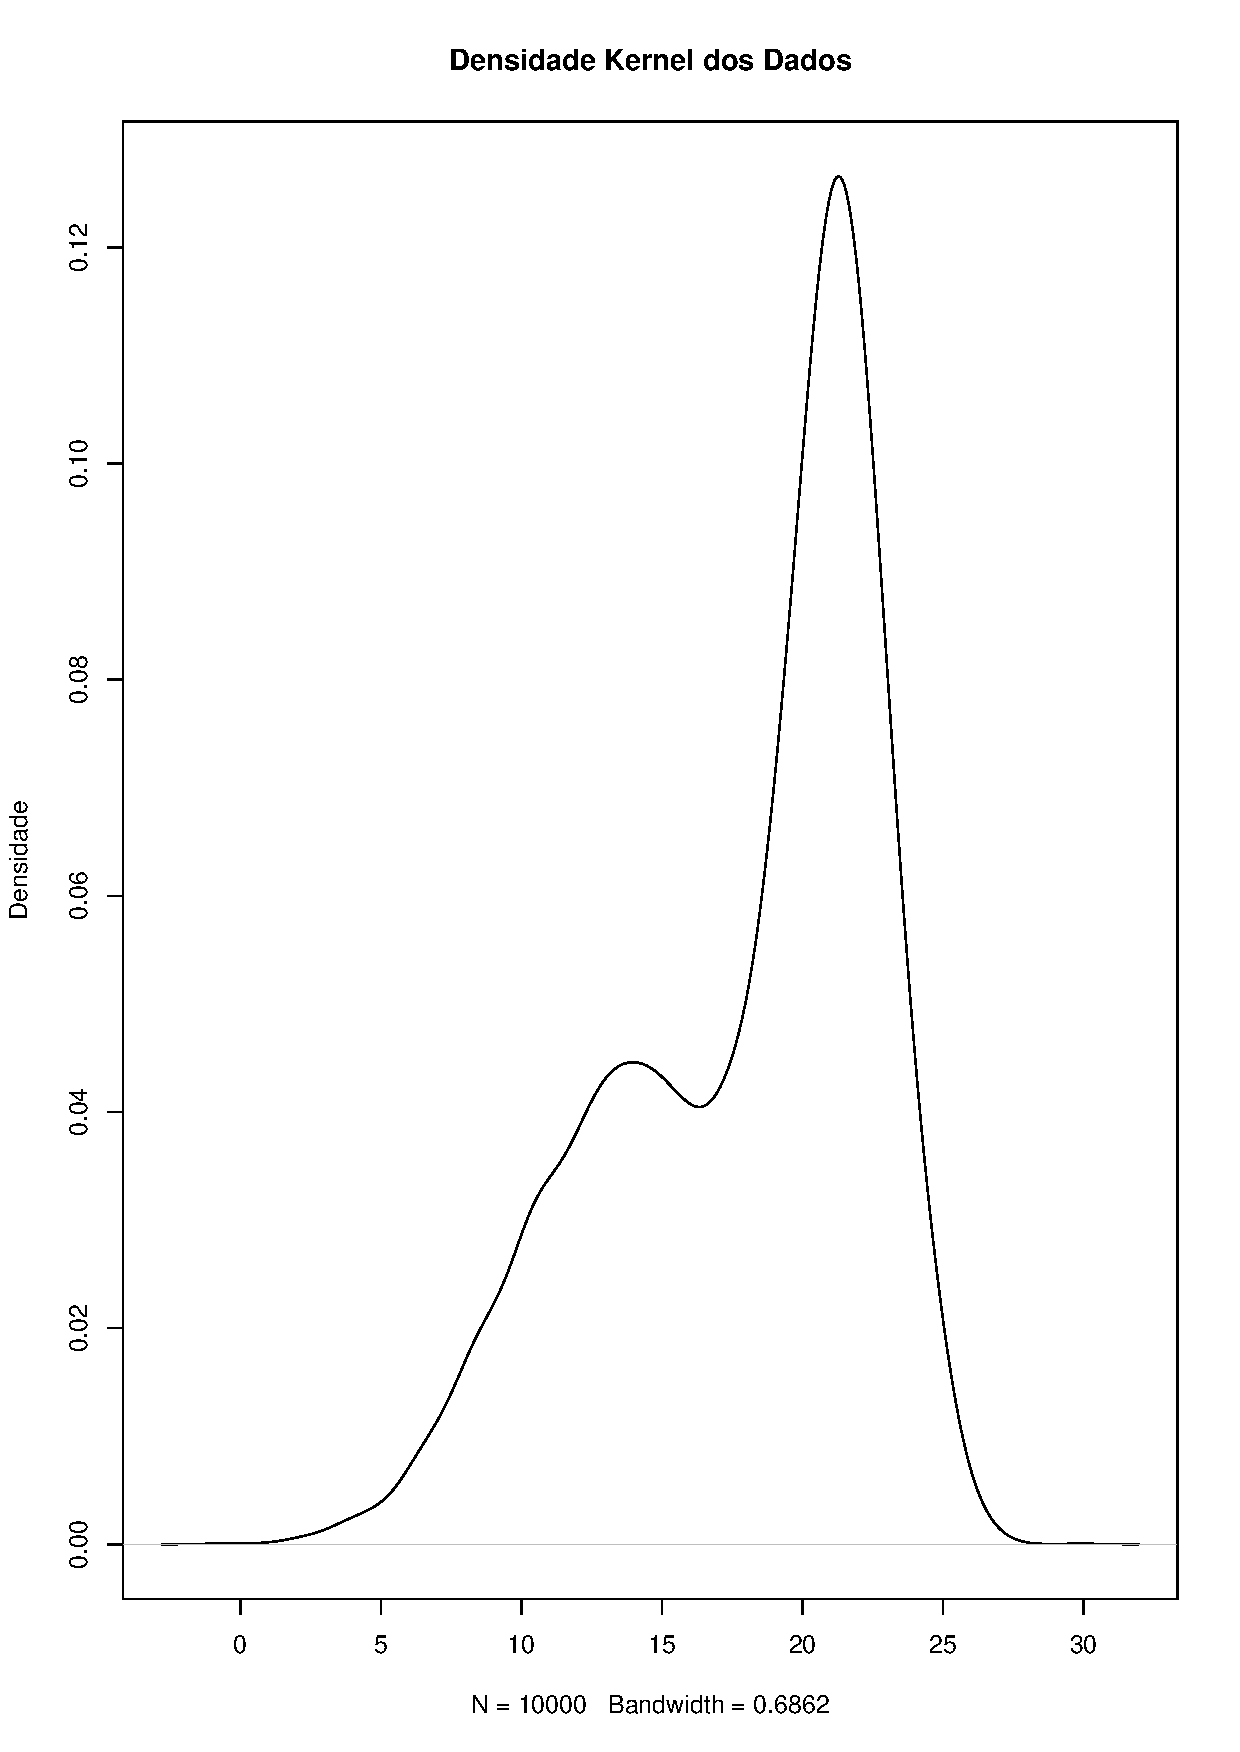
\includegraphics[scale = 0.6]{exp1}
\caption{istribuição dos dados disponibilizados}
\label{fig:exp1}
\end{figure}



\begin{table}
	\centering
	\begin{tabular}{c|c}
	Estatística & Valor \\\hline
    Mínimo & $-0,7261$ \\
    1o Quartil & 14,4100 \\
    Mediana & 19,5600 \\
    Média & 17,9700 \\
    3o Quartil & 21,6500 \\
    Máximo & 29,9000 \\
    Desvio-padrão & 4,811046\\
    Assimetria & $-0.7471169$ \\
    Curtose & 2.682648
  	\end{tabular}
    \caption{Estatísticas descritivas para os dados disponibilizados}
    \label{tab:1}
\end{table}

Por inspeção, a distribuição dos dados é bimodal, discretamente assimétrica e leptocúrtica, pois sua Curtose é positiva. Uma análise exploratória longa e detalhada não é estritamente necessária, ainda mais se tratando de problema com interesse acadêmico e dados já conhecidamente vindos de uma mistura de distribuições normais.


O Algoritmo EM implementado em \ref{anexo:a} foi aplicado a quatro conjuntos de estimativas para os valores inciais, descritos na Tabela \ref{tab:2}. As escolhas dos três primeiros conjuntos de estimativas é arbitrária, a do quarto conjunto é livremente inspirada pela Tabela \ref{tab:1}, e pela Figura \ref{fig:exp1}.

\begin{table}[H]
	\centering
	\begin{tabular}{c|ccccccc}
   	Subconjunto &$\hat{p}$ & $\hat{\mu_1}$ & $\hat{\mu_2}$ & $\hat{\sigma_1}$ & $\hat{\sigma_2}$ \\\hline
    \textbf{1} & 0,5& $X_{(1)}$ = $-0,7261$ & $X_{(n)}$ = $29,9000$ & s(X) = 4,811046 & s(X) = 4,811046\\
    \textbf{2} &0,1& 0 & 100 & 4,811046 & 4,811046 \\
    \textbf{3} &0,5 &6 & 21 & 1 & 1 \\
    \textbf{4} & 0,4 & 14 & 22 & 8 & 4 \\


  	\end{tabular}
    \caption{Estimativas iniciais para os parâmetros a serem utilizados pelo Algoritmo EM}
    \label{tab:2}
\end{table}


\section{Resultados}
\label{sec:resultados}
A Tabela \ref{tab:3} contém as estimativas obtidas pelo Algoritmo EM para os parâmetros envolvidos na mistura de duas distribuições gaussianas. Note como o primeiro subconjunto de prováveis resultados sequer convergiu: escolher o mínimo e o máximo das observações como possíveis estimativas iniciais para as médias provou-se catastrófico. A Figura \ref{fig:estimativas} ilustra separadamente as distribuições obtidas utilizando os parâmetros estimados pelo Algoritmo EM. Note como nos dois primeiros casos as estimativas são grosseiras, inclusive para o Subconjunto 3 as curvas têm comportamento "trocado". A melhor estimativa é a obtida para o subconjunto 4, e uma mistura de normais com 10000 observações e as respectivas proporções para os parâmetros é dada na Figura \ref{fig:sub4}.

\begin{table}[H]
	\centering
	\begin{tabular}{c|ccccccc}
   	 & $\hat{p}$ & $\hat{\mu}_1$ & $\hat{\mu}_2$ & $\hat{\sigma}_1^2$ & $\hat{\sigma}_2^2$ & iterações \\\hline
    \textbf{1} & \multicolumn{5}{c}{\textbf{Não convergiu}} & NA\\
    \textbf{2} & 0.005215596 & 12.218441927 & 17.996614181 & 27.519357947 & 22.946778066 & 427 \\
    \textbf{3} & 0.2099091 & 10.3834012 & 19.9811271 & 5.5454028 & 8.4833039 & 1703\\
    \textbf{4} & 0.4264324 & 13.3639992 & 21.3882995 & 13.1367257 & 3.1261634 & 2083
  	\end{tabular}
    \caption{Estimativas obtidas pelo Algoritmo EM para os respectivos subconjuntos}
    \label{tab:3}
\end{table}

\begin{figure}[H]
\centering
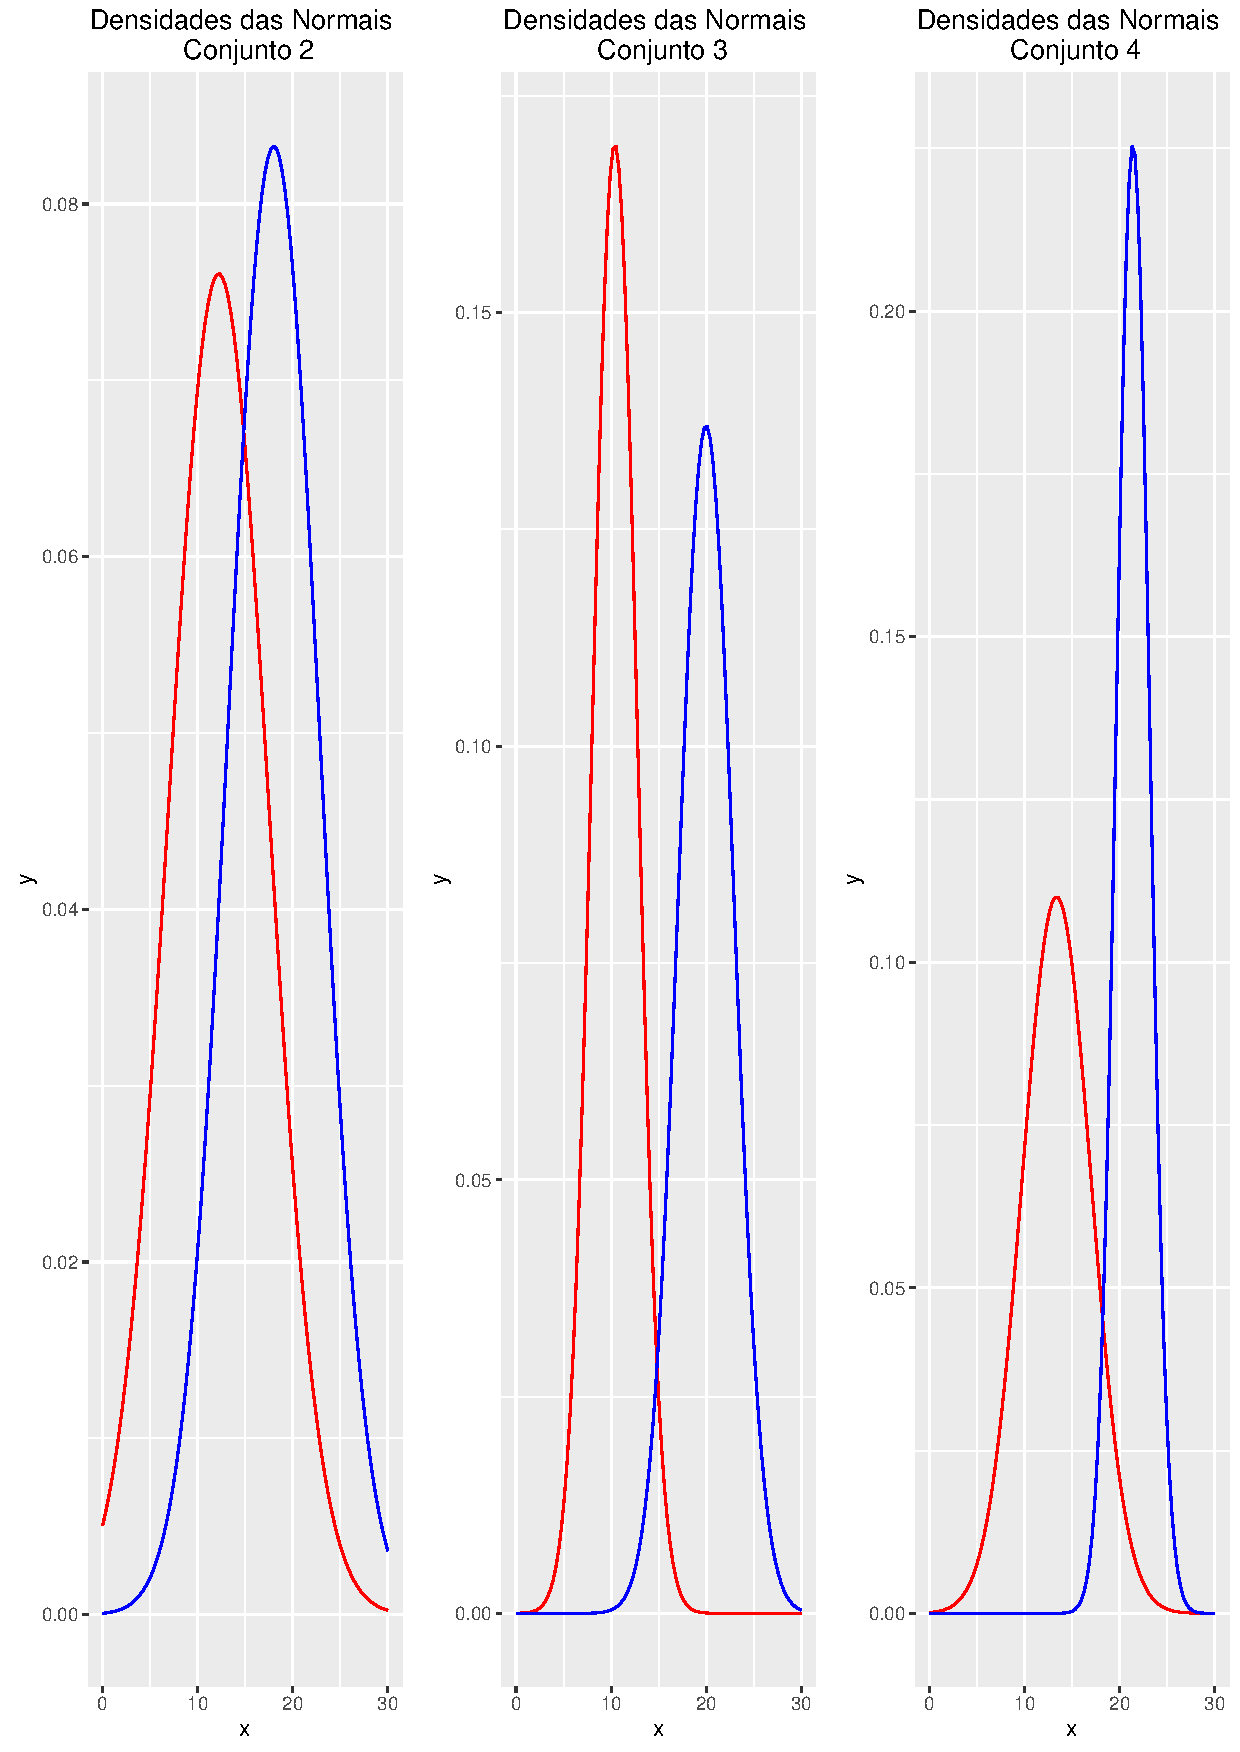
\includegraphics[height = 8cm, width = 16cm]{estimativas}
\caption{Gráficos para a distribuição dos dados segundo as estimativas para os parâmetros obtidas pelo Algoritmo EM}
\label{fig:estimativas}
\end{figure}


\begin{figure}[H]
\centering
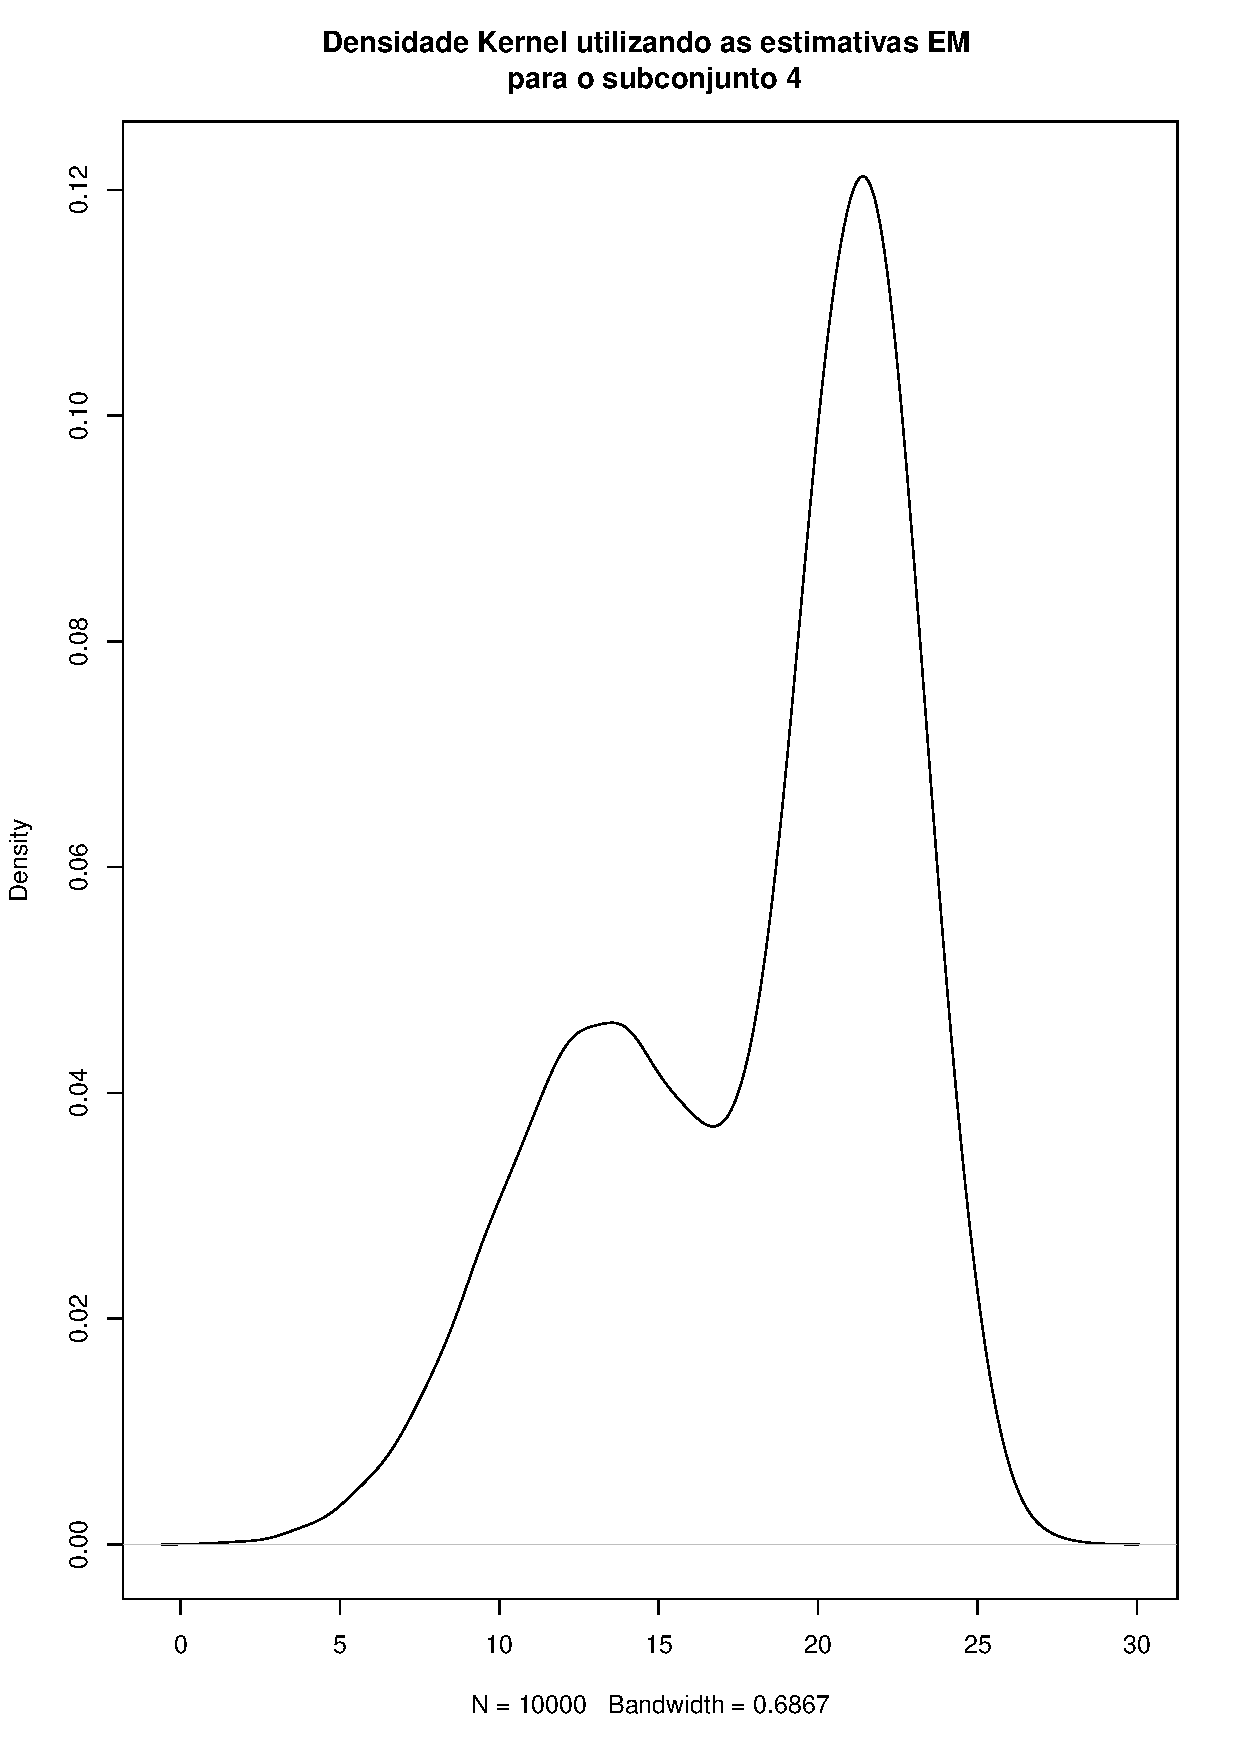
\includegraphics[scale = 0.6]{sub4}
\caption{Gráficos para a distribuição dos dados segundo as estimativas para os parâmetros obtidas pelo Algoritmo EM}
\label{fig:sub4}
\end{figure}

\section{Conclusões}
\label{sec:conclusoes}
A etapa de Análise Descritiva mostrou-se essencial. As estimativas obtidas para o Subconjunto 4 mostraram-se graficamente \textit{boas o suficiente}, e a melhor inspeção que podemos fazer nesse caso é desse tipo, já que qualquer Teste de Aderência rejeitaria a hipótese de identidade entre a distribuição dos dados disponibilizados e uma distribuição gerada aleatoriamente com os parâmetros estimados pelo Algoritmo EM. O Teste de Kolmogorov-Smirnov, por exemplo, rejeita a hipótese nula com significância de 0,07555. 
\bookmarksetup{startatroot}% 




% ----------------------------------------------------------
% ELEMENTOS PÓS-TEXTUAIS
% ----------------------------------------------------------
\postextual



% ----------------------------------------------------------
% Referências bibliográficas
% ----------------------------------------------------------
\bibliography{tp5-ref}


\cftinserthook{toc}{AAA}
% ---
% Inicia os anexos
% ---
%\anexos
\begin{anexosenv}

% ---
\chapter{Implementação do Algoritmo na linguagem R}
\label{anexo:a}

O código-fonte deste trabalho encontra-se disponível no repositório \url{https://github.com/august-o/TP5-EstComp}.

A implementação não conta com nenhuma limitação óbvia, mas a função \texttt{iteracao()} poderia ser mais versátil, utilizando as capacidades de vetorização de funções do R e não laços e condições lógicas. Como o Algoritmo EM é \textit{relativamente eficiente}\footnote{Expressão utilizada em sentido livre, já que, por ser um Método Iterativo, sua Ordem pode ser $\infty$}, as estimativas foram obtidas quase instantaneamente para o conjunto de dados disponibilizados, cujo tamanho era considerável (n = 10000). Outros tamanhos foram testados \textit{ad hoc} para verificar a convergência do algoritmo, como n = 1000000 e n = 100000000, e ainda assim o método convergiu em poucos minutos.

\lstset{inputencoding=utf8/latin1}
\lstinputlisting[language=R]{TP5.R}

\end{anexosenv}

\end{document}